\documentclass{article}           % Sets style/look of many things.
% \documentclass{report}          % part, chapters, front page etc.
\usepackage{exsheets}
\usepackage[utf8]{inputenc}       % Encoding of input files UTF-8
\usepackage[T1]{fontenc}
\usepackage[scaled]{beramono}     % Font
\usepackage{color}                % Color text
\usepackage{titlesec}             % Select alternative section titles
\usepackage{fancyvrb}
\usepackage{verbatim}             % Comment environment
\usepackage{listings}             % Format and render text/code etc.
\usepackage{minted}               % Much better syntax highlighting
\usepackage{float}                % Control of floating environment/figure
\usepackage{graphicx,  subfigure} % Better figures, graphics, units etc.
\usepackage{multicol}             % Multiple columns
\usepackage{amsmath}              % Math: Equation, split, align etc.
\usepackage{siunitx}              % SI units
\usepackage{mathtools}            % Different math tools to use with amsmath
\usepackage{amssymb}              % Math symbols
\usepackage[
    colorlinks,
    citecolor=black,              % I like links with standard black color
    filecolor=black,
    linkcolor=black,
    urlcolor=black
]{hyperref}                       % Links in TOC etc.
\usepackage[all]{hypcap}          % Better links to floating environment

\usepackage{tabto}
\newcommand\marginsymbol[1][0pt]{%
    \tabto*{0cm}\makebox[\dimexpr-1cm-#1\relax][r]{$\mathbb{P}$}\tabto*{\TabPrevPos}}

\renewcommand{\thesubsection}{\thesection.\alph{subsection}}

% Make margins smaller to fit more figures, tables etc on page: (optional)
\addtolength{\oddsidemargin}{-1.0in}
\addtolength{\evensidemargin}{-1.0in}
\addtolength{\textwidth}{2.0in}
\addtolength{\topmargin}{-0.8in}
\addtolength{\textheight}{1.6in}

\title{\vspace{-2cm}INF3490/INF4490 Exercises - Unsupervised Learning}
\author{Eivind Samuelsen\footnote{See \href{https://github.com/olehermanse/INF3490-AI_Machine_Learning/blob/master/README.md}{\textbf{README}} for complete list of authors/contributors.}
}
\date{}

% Removing paragraph indents is sometimes useful:
\setlength\parindent{0pt}
% ==============================================================================

% ================================= DOCUMENT ===================================
\begin{document}
    \renewcommand\marginsymbol[1][0pt]{%
  \tabto*{0cm}\makebox[-1cm][c]{$\mathbb{P}$}\tabto*{\TabPrevPos}}

\maketitle
\(\mathbb{P}\) marks the programming exercises, we strongly recommend using
the python programming language for these. Exercises may be added/changed
after publishing.


\section{k-means clustering}
The following graph shows 2D data points. It is clear from the graphs that there are two clusters. Will \(k\)-means clustering be able to find these two, if we define \(k = 2\)? If not, why?
\begin{figure}[H]
\begin{center}
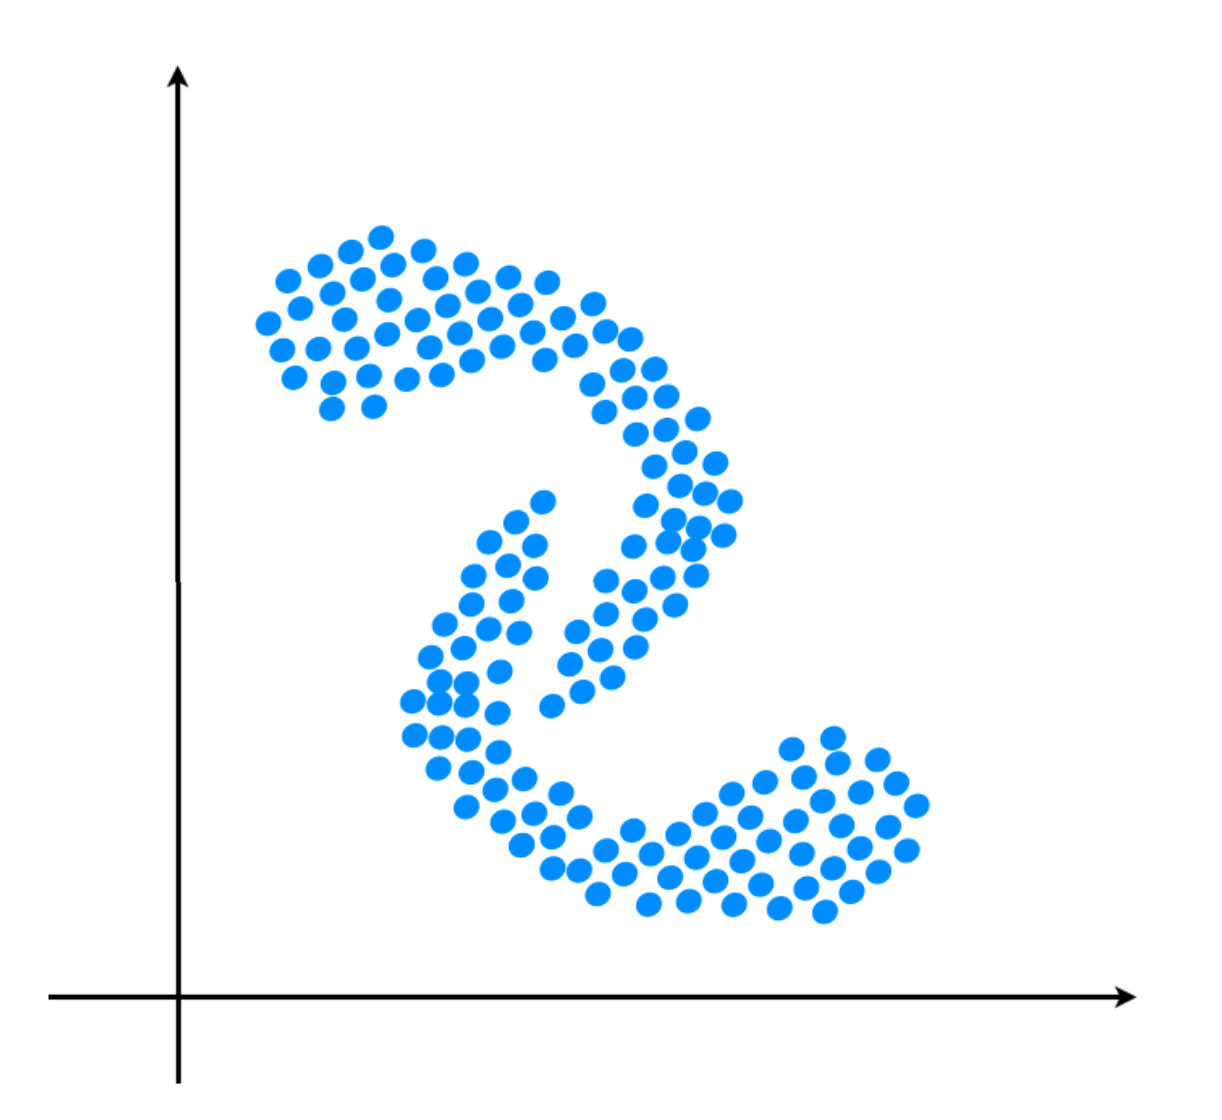
\includegraphics[width=0.6\textwidth]{two_clusters.png}
\end{center}
\end{figure}

\section{Self organizing maps}
In SOMs, what role do the predefined topological (neighborhood) relationships between neurons in the map space play in the discovery of topological (neighborhood) relationships between input vectors in the data space?

\section{Gaussian function in SOMs}
In SOMs, a Gaussian function, as defined below, can be used to define the neighborhood relation
\begin{equation}
N(i,j) = e^{-\frac{||i-j||^2}{2\sigma^2(t)}}
\end{equation}
where \(i\) and \(j\) are two neurons, whose position on the lattice are given by (row, columnt), and \(||i-j||\) is the Euclidian distance between them. So, if \(i\)'s position is \((2,2)\) and \(j\)'s position is \((3,3)\) and \(\sigma(t) = 1\), \(N(i,j)\) will be \(e^{-1}\).

As can also be seen, the further a neuron \(i\) is from the winning neuron \(j\) on the lattice the smaller \(N(i,j)\) is. What would happen if \(N(i,j)\) is set to and remains zero for all neurons except the winning neuron? What would happen if \(N(i,j)\) is set to and remains 1 for all neurons including the winning neuron? Why is it important to have \(N(i,j)\) large for distant (on the lattice/map space) neurons in the beginning of the learning process i.e. \(j\) should have a larger neighborhood, and smaller as time goes by? This can be controlled by \(\sigma(t)=\sigma_0e^{-t/T}\), where \(\sigma_0\) is the initial value of \(\sigma\), and \(T\) is a constant.

Example Matlab script that can be run to see how the neighborhood funcion may change with time:
\begin{figure}[H]
\begin{center}
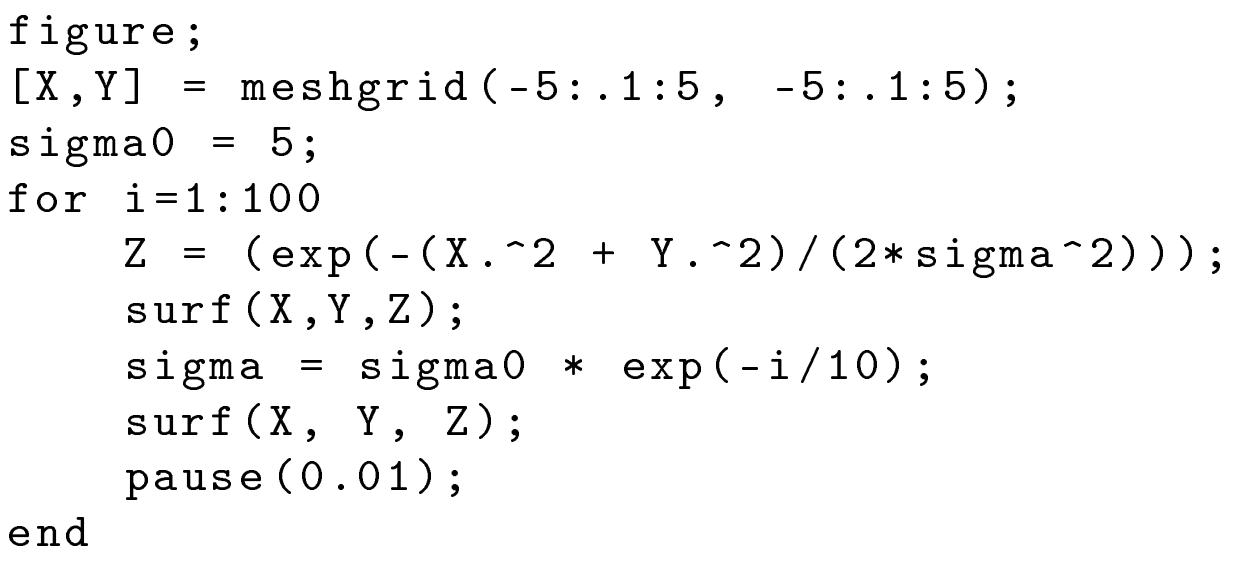
\includegraphics[width=0.6\textwidth]{matlab_example.png}
\end{center}
\end{figure}

Describe one other neighborhood relationship function that can be used for SOMs. In what way can it influence the learning process? Explain.

\section*{Contact and Github}
Corrections of grammar, language, notation or suggestions for improving this material are appreciated.
E-mail me at \href{mailto:olehelg@uio.no}{\textbf{olehelg@uio.no}} or use \href{https://github.com/olehermanse/INF3490-AI_Machine_Learning}{\textbf{GitHub}} to submit an issue or create a pull request.
The \href{https://github.com/olehermanse/INF3490-AI_Machine_Learning}{\textbf{GitHub repository}} contains all source code for assignments, exercises, solutions, examples etc.
As many people have been involved with writing and updating the course material, they are not all listed as authors here.
For a more complete list of authors and contributors see the \href{https://github.com/olehermanse/INF3490-AI_Machine_Learning/blob/master/README.md}{\textbf{README}}.

\end{document}
% ==============================================================================
